\section{GoTxn's specification}

At a high level, GoTxn makes transactions atomic. We frame its specification in
two ways. The first, \emph{program refinement}, formalizes the idea of ``atomic
transactions'' more literally. The second, \emph{simulation transfer} uses
program refinement to show that a sequential proof of a system's transactions
implies the concurrent system is correct running on top of GoTxn.

At a high level, GoTxn's specification says that transactions execute
atomically. The way this is stated formally is by considering an arbitrary
caller, a program that has transactions using the GoTxn API. Then correctness is
defined by relating this executable code to an abstract, specification program,
a version of the caller code where the GoTxn methods are treated as primitives.
An important aspect of GoTxn is that the specification program is defined using
an atomic block around each transaction, whose semantics is to run the body
without interleaving other threads.

Before we can get to defining these specification programs, we first set up
\emph{refinement}, which is the relationship between the code and spec.
Abstractly, refinement from a code program to
a specification program says that the behaviors of the code are a subset of the
behaviors of the specification.

To define the specification, we need to be more precise about what a program is
and how it executes to talk about the server loop program. We
write $p : \gooselayer{X}$ to say $p$ is a Go program written using operations
from layer X, where X is one of NFS, Txn, or Disk.
Layer operations are always atomic transitions in a state machine. In the
NFS layer, the operations behave according to the NFS state machine
described previously in \cref{sec:spec} and defined formally in Dafny.
The Txn layer is specified both in Coq where it is part of the transaction
system's correctness theorem and in Dafny where it appears as an assumption. The
Disk transition system is formalized in Coq as part of the GoJournal proof,
and assumes reads and writes of 4KB blocks are atomic. Each layer
includes concurrent threads that interleave layer
operations, basic heap operations on pointers, slices, and maps, and computation
on primitives like integers and structs.

There are three programs involved in defining and proving the overall
correctness of \sys, corresponding to the server loop at each abstraction layer.
At the top, the specification is a loop $\snfs : \gooselayer{NFS}$ which
atomically processes each NFS operation according to the NFS state machine. The
next level is $\sdfy : \gooselayer{Txn}$, where each handler is the atomic body of the
corresponding Dafny method, operating on top of the transaction system. Finally,
the executable code is written
$\mathrm{link}(\sdfy, \txncode) : \gooselayer{Disk}$, indicating ``linking'' the
Txn-layer server $\sdfy$ with the transaction system by taking each call to a
Txn API and plugging in its implementation on top of a disk.
\Cref{fig:refinement-execs} illustrates one execution of the DaisyNFS server,
when clients issue a \cc{LOOKUP} and \cc{CREATE} in parallel; for correctness,
the operations should be atomic and follow the NFS specification despite
interleaving at the code level (the bottom execution).

In the Txn layer, we write $\atomically{\cc{f}}$ to represent a
transaction running \cc{f}. This is a macro that expands to a
sequence like \cc{tx := Begin(); f(tx); tx.Commit()} (some additional code
handling aborts is omitted in this snippet).
% At the specification
% level, an atomically block represents a whole sequence of operations that
% executes all at once, without crashes or other threads interrupting.

\begin{figure}
  %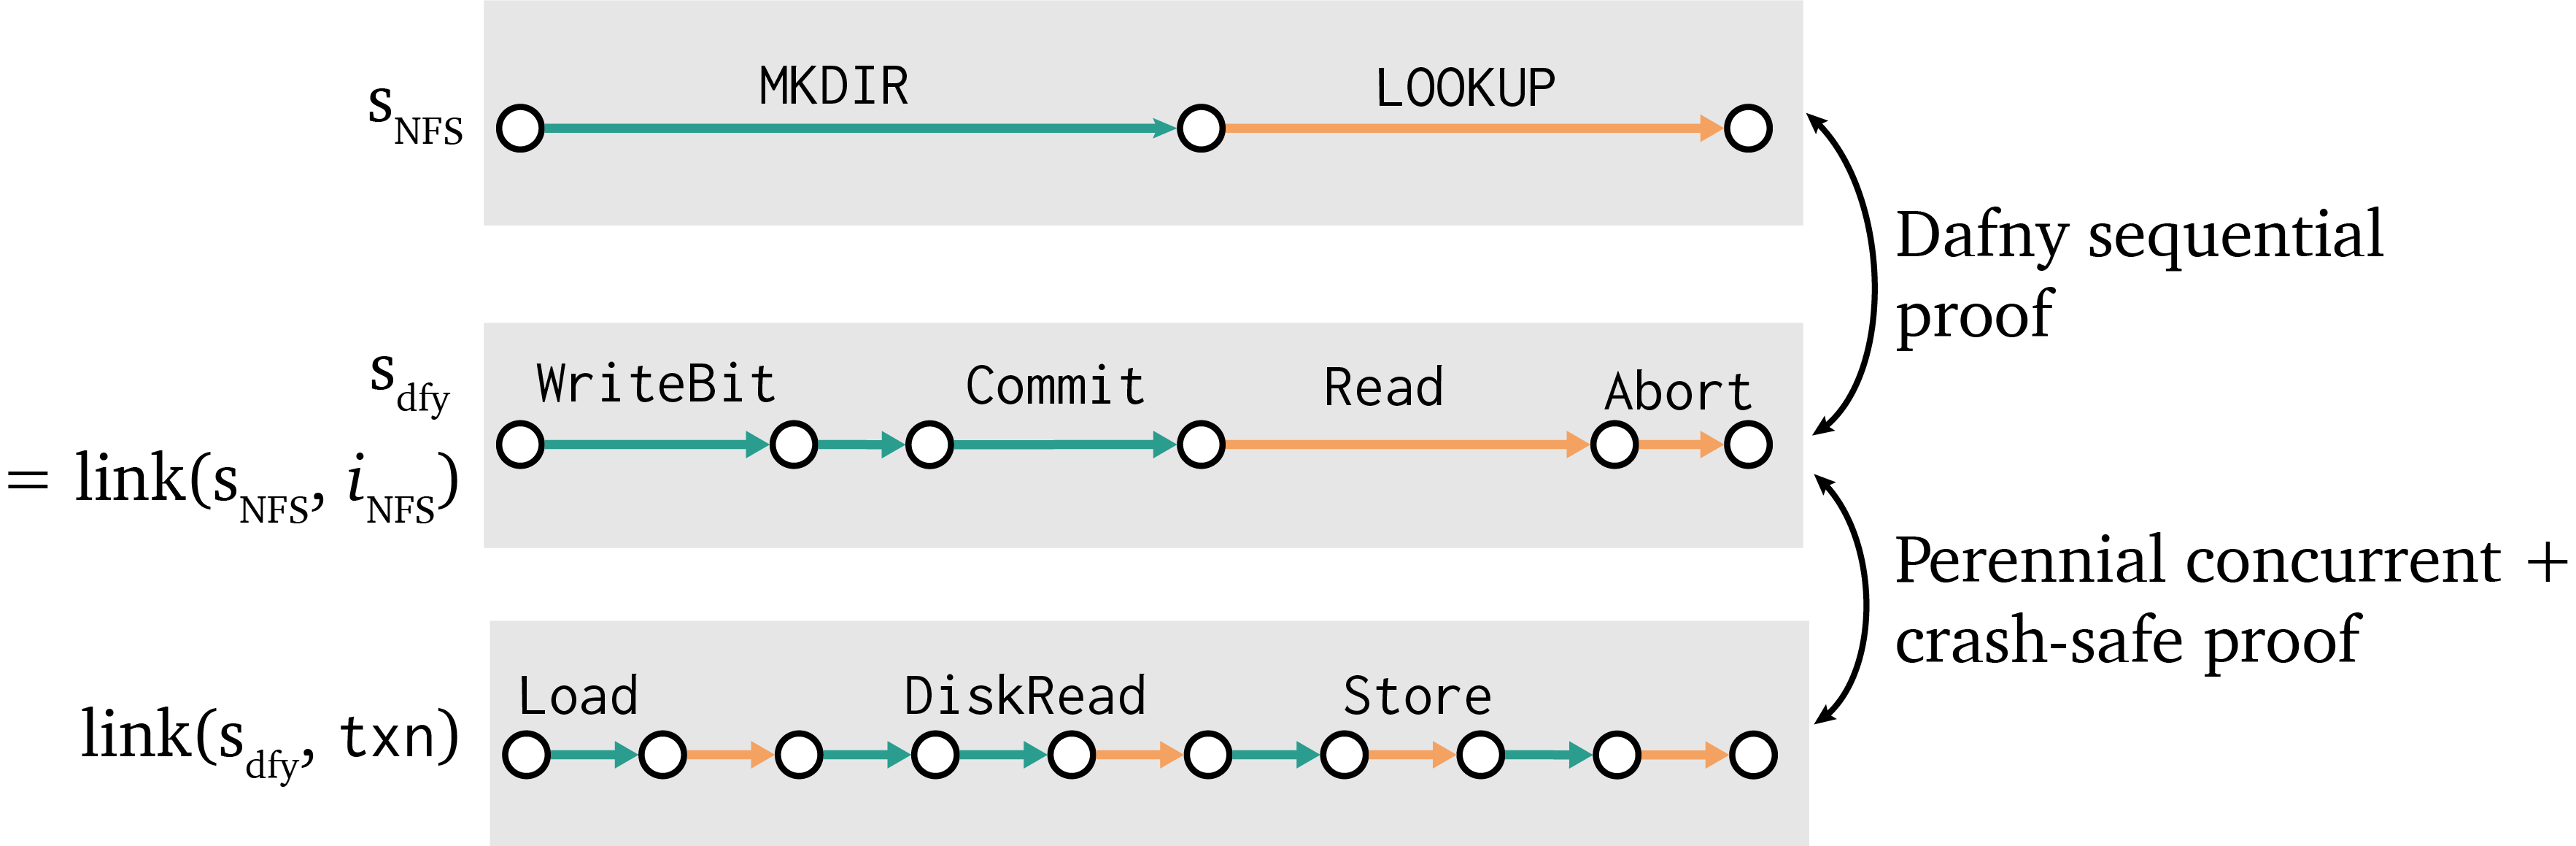
\includegraphics{fig/refinement-execs}
  \begin{center}
  \begin{tikzpicture}[scale=1, >=latex, every node/.append style={}]

  \tikzstyle{txnstate}=[circle,draw,minimum size=2mm,fill=blue!10]
  \tikzstyle{nfsstate}=[circle,draw,minimum size=2mm,fill=yellow!10]
  \tikzstyle{diskstate}=[circle,draw,minimum size=2mm,fill=green!10]
  \tikzstyle{switch}=[->, dashed, dash pattern=on 1.5pt off 2pt]
  \tikzstyle{stepr}=[thick,->]
  \tikzstyle{layer}=[font=\large]

  \setlength{\stepw}{1.25cm}
  \setlength{\dstepw}{\stepw*2}

  \newlength{\nfsbot}
  \newlength{\nfsmid}
  \setlength{\nfstop}{1.5cm}
  \setlength{\nfsbot}{.5cm}
  \setlength{\nfsmid}{(\nfstop+\nfsbot)/2}

  \newlength{\txntop}
  \newlength{\txnbot}
  \newlength{\txnmid}
  \setlength{\txntop}{-.5cm}
  \setlength{\txnbot}{-1.5cm}
  \setlength{\txnmid}{(\txntop+\txnbot)/2}

  \newlength{\disktop}
  \newlength{\diskbot}
  \newlength{\diskmid}
  \setlength{\disktop}{-2.5cm}
  \setlength{\diskbot}{-3.5cm}
  \setlength{\diskmid}{(\disktop+\diskbot)/2}

  \draw node (N0a) at (0,\nfstop) [nfsstate] {};
  \draw node (N1a) at (\dstepw,\nfstop) [nfsstate] {};
  \draw node (N1b) at (\dstepw,\nfsbot) [nfsstate] {};
  \draw node (N2b) at (\dstepw*2,\nfsbot) [nfsstate] {};

  \draw [stepr] (N0a.east) -- (N1a.west) node[midway,above=.2] {\code{LOOKUP}};
  \draw [stepr] (N1b.east) -- (N2b.west) node[midway,above=.2] {\code{CREATE}};
  \draw [switch] (N1a.south) -- (N1b.north);

  \draw node (T0a) at (0,\txntop) [txnstate] {};
  \draw node (T1a) at (\stepw,\txntop) [txnstate] {};
  \draw node (T2a) at (\stepw*2,\txntop) [txnstate] {};
  \draw node (T2b) at (\stepw*2,\txnbot) [txnstate] {};
  \draw node (T3b) at (\stepw*3,\txnbot) [txnstate] {};
  \draw node (T4b) at (\stepw*4,\txnbot) [txnstate] {};

  \draw [stepr] (T0a.east) -- (T1a.west) node[midway,above=.2] {};
  \draw [stepr] (T1a.east) -- (T2a.west) node[midway,above=.2] {\code{Commit}};
  \draw [switch] (T2a.south) -- (T2b.north);
  \draw [stepr] (T2b.east) -- (T3b.west) node[midway,above=.2] {};
  \draw [stepr] (T3b.east) -- (T4b.west) node[midway,above=.2] {\code{Abort}};

  \draw node (D0a) at (0,\disktop) [diskstate] {};
  \draw node (D1a) at (\stepw,\disktop) [diskstate] {};
  \draw node (D1b) at (\stepw,\diskbot) [diskstate] {};
  \draw node (D2b) at (\stepw*2,\diskbot) [diskstate] {};
  \draw node (D3b) at (\stepw*3,\diskbot) [diskstate] {};
  \draw node (D3a) at (\stepw*3,\disktop) [diskstate] {};
  \draw node (D4a) at (\stepw*4,\disktop) [diskstate] {};

  \draw [stepr] (D0a.east) -- (D1a.west) node[midway,above=.2] {\code{Read}};
  \draw [switch] (D1a.south) -- (D1b.north);
  \draw [stepr] (D1b.east) -- (D2b.west) node[midway,above=.2] {\code{Write}};
  \draw [stepr] (D2b.east) -- (D3b.west) node[midway,above=.2] {};
  \draw [switch] (D3b.north) -- (D3a.south);
  \draw [stepr] (D3a.east) -- (D4a.west) node[midway,above=.2] {};

  \draw [align=center] node (NFS) at (\stepw*5.5,\nfsmid) [layer] {$\snfs$ \\ \gooselayer{NFS}};
  \draw [align=center] node (Txn) at (\stepw*5.5,\txnmid) [layer] {$\sdfy$ \\ \gooselayer{Txn}};
  \draw [align=center] node (Disk) at (\stepw*5.5, \diskmid) [layer] {$\linkedcode$ \\ \gooselayer{Disk}};

\end{tikzpicture}

  \end{center}
  \vspace{-\baselineskip}
  \caption{One possible execution of DaisyNFS, receiving parallel LOOKUP and
    CREATE operations, at its three abstraction levels.
    Within an execution each row is a thread, and dashed arrows indicate
    context switches.
    The proof shows the bottom execution is equivalent to an atomic execution of
    each thread at
    the Txn layer~(in \cref{thm:gotxn}),
    and sequential reasoning shows each atomic sequence behaves according to the NFS
    specification~(in \cref{thm:dafny}).}
  \label{fig:refinement-execs}
\end{figure}

Refinement relates two programs in terms of their visible behavior, which we
will use to connect the server loop at the disk layer to the transaction layer
and finally to the NFS layer. For the purposes of this paper, all of the
programs involved are servers that issue network I/O, either receiving an NFS
request or responding to one. Regardless of the level of abstraction, each model
of the server defines a trace of network I/O consisting of requests and
responses, and this is the behavior refinement talks about:

\begin{definition}[Refinement]
  An implementation program $p_{c}$ refines a specification program $p_{s}$,
written $p_{c} \refines p_{s}$, if whenever there are initial states
$\sigma_{s}$ and $\sigma_{c}$ satisfying $\mathrm{init}(\sigma_{s}, \sigma_{c})$
and $p_{c}$ can execute from $\sigma_{c}$ and produce a trace of network I/O
$tr$, then $p_{s}$ can execute from $\sigma_{s}$ and produce the same trace
$tr$.  Execution might involve crashing and restarting a program (potentially
multiple times), wiping out any in-memory state after each crash.
  \label{def:refinement}
\end{definition}

The intuition behind the notation $p_{c} \refines p_{s}$ is that the set of
behaviors of $p_{c}$ (the set of traces of network I/O $tr$) is a subset of the
behaviors of $p_{s}$. Whenever we state $p_{c} \refines p_{s}$ we leave implicit
a definition of initial states $\mathrm{init}(\sigma_{s}, \sigma_{c})$, which
will generally say both states are all zeros and of the same size.

\subsection{Program refinement}

We define the correctness of the transaction system's implementation as a
\emph{program refinement}.
To set up this specification, consider a program $p : \gooselayer{Txn}$ that
uses transactions.
To run $p$, it is combined with the transaction-system implementation, producing
a program $\mathrm{link}(p, \txncode) : \gooselayer{Disk}$ that can be run on
top of a disk.
Transactions in the linked program continue to have the expected atomic
behavior, so long as transaction code in $p$ follows certain restrictions, such
as not accessing shared state outside the journal system.  We write
$\mathrm{safe}(p)$ to mean $p$ is ``safe'' in the sense that it follows these restrictions.

% At a high level of abstraction, the main difficulty is to give a specification
% for the transaction system, which we do in several steps:
%
% \begin{enumerate}
%   \item First, we define an arbitrary Go program running on top of
%         the transaction system. For reasons we will explain shortly we will use
%         $p : \gooselayer{Txn}$ for such a program. To run such a program it
%         first needs to be linked with the transaction system implementation,
%         producing a program denoted $\mathrm{link}(p, \txncode)$.
%   \item The second idea is to say what the semantics of a program
%         $p : \gooselayer{Txn}$ is. Transactions are atomic in this semantics in
%         that the whole transaction transitions at once, without interleaving
%         other threads. The program can issue reads and writes within a
%         transaction, and they follow a simple state machine.
%   \item The final idea is to define ``safe'' programs $\mathrm{safe}(p)$, those
%         that follow the restrictions of the transaction system. The
%         specification only applies to safe programs.
% \end{enumerate}

The correctness of the transaction system is summarized by the following theorem:

\begin{theorem}
  The transaction system's implementation $\txncode$ is a program refinement, meaning for
  all $p : \gooselayer{Txn}$, if $\mathrm{safe}(p)$, then
  $\mathrm{link}(p, \txncode) \refines p$. The definition of
  $init(\sigma_{s}, \sigma_{c})$ in this refinement relates an all-zero physical
  disk to an all-zero transactional disk of the same size.
  \label{thm:gotxn-program-refinement}
\end{theorem}

\Cref{thm:txn} is stated in Coq and has a fully mechanized proof in Perennial.
What it says is that if a program is safe, the program linked with the
transaction system always behaves as if its transactions were atomically
accessing a transactional disk logically maintained by the transaction system.
The definition of safety formalized in Coq requires that code within a
transaction not access any shared memory outside of the transaction layer; other
than that, transactions are permitted to issue reads, writes, and do other
computation. Safety also requires that transactions follow the preconditions of
the \cc{Read} and \cc{Write} operations, which require a discipline of accessing
each object with a fixed size. Finally, safe programs can only \cc{Abort} or
\cc{Commit} a given transaction once. The notion of safe program will be
important when linking this proof with the Dafny proofs, since the transaction
system's proof only applies to a safe caller.

\subsection{Simulation transfer}

The idea behind the transaction-system specification is to express that a system
verified using sequential reasoning for each transaction is also correct when
run concurrently through GoTxn --- intuitively, this follows from the fact that
transactions appear to run atomically.
% , at which point the sequential reasoning
% applies, but we have a more precise and formal proof in Coq.
To make this precise, we define formally what we mean by
``sequential reasoning''. Suppose we have an
implementation of layer $S$ using operations from $T$. Note that all the proofs
about the transaction system are for an arbitrary system with operations in $S$;
Though we use the system with an implementation of NFS, its proof is
more general. The implementation $i$
consists of a function $i(op) : \gooselayer{T}$ for each operation $op \in S$. The statement
$\seqrefinement \targ{T, S}(i)$ says that $i$ is a correct sequential
implementation of $S$ using $T$. To specify correctness under crashes, this
definition refers to $\operatorname{crash}(\sigma, \sigma')$, which is a
layer-specific crash transition that models, for example, clearing the
contents of memory.

\begin{definition}
  The implementation $i : S \to \gooselayer{T}$ is a \emph{sequential
    refinement}, written
  $\seqrefinement \targ{T, S}(i)$, if there exists an abstraction relation
  $R : \Sigma_{S} \to \Sigma_{T} \to bool$ such that: \newline
(1) for every operation
  $op \in S$, the following sequential Hoare triple holds:
  \[
    \hoare{R(\sigma)}{i(op)}{\exists \sigma'.\, R(\sigma') \land \sigma \overset{op}{\leadsto} \sigma'},
  \]
(2) $\mathrm{init}(\sigma_{S}, \sigma_{T})$ must imply
$R(\sigma_{S}, \sigma_{T})$, and \\
(3) if $R(\sigma_{T}, \sigma_{S})$ holds and $\operatorname{crash}(\sigma_{T}$, $\sigma_{T}')$,
then there exists a $\sigma_{S}'$ such that $R(\sigma_{T}', \sigma_{S}')$ and
$\operatorname{crash}(\sigma_{S}, \sigma_{S}')$.%
  \label{def:seqrefinement}
\end{definition}
%
Conditions (1) and (2) in this definition are standard for sequential
verification of refinement, while condition (3) is a standard condition for sequential crash-safety~\citep{chajed:argosy}. Though condition (3) requires the
abstraction relation to be preserved by crashes, the proof engineer does \emph{not} have to reason about crashes in the middle of operations.
% is a standard condition for sequential crash-safety~\cite{chajed:argosy}
% for sequential crash safety~\cite{chajed:argosy}.
The
diagram in \cref{fig:refinement} depicts the main
refinement condition (1) diagrammatically.
% For example, it is fairly easy to use them to show
% that for any sequential program $p : \gooselayer{S}$, the traces of the code
% $\mathrm{link}(p, i)$ are a subset of the traces of the spec $p$ (we will not
% use exactly this theorem since we are interested in concurrent code using
% transactions).
% \tej{I mentioned this but maybe we don't want/need to say it?}. Such reasoning would be familiar in previous sequential verified
% systems like FSCQ~\cite{chen:fscq}, IronFleet~\cite{hawblitzel:ironfleet}, and
% VeriBetrKV~\cite{hance:veribetrkv}.

The correctness theorem for GoTxn takes a proof of \emph{sequential} refinement
conditions for a system implemented using transactions and derives a \emph{concurrent and crash-safe} refinement.
A transaction must satisfy some conditions to ensure atomicity. We write
$\mathrm{safe}(p)$ to say that $p$ is a valid transaction. The main
restriction is that $p$ cannot access global state such as the heap, since
the transaction system does not make such accesses atomic.
The implementation $i$
in this theorem gives only the body of each transaction; the theorem is about
$\atomiccomp i$ where $(\atomiccomp i)(op) = \atomically{i(op)}$ uses
the macro from the Txn layer to specify that the
operation is wrapped in a transaction.
%\begin{verbatim}
%type txnBody =
%  func(tx *Txn) (v interface{}, ok bool)
%func runTxn(f txnBody) (v interface{}, ok bool) {
%  tx := Begin()
%  v, ok := f(tx)
%  if ok {
%    tx.Commit()
%  } else {
%    tx.Abort()
%  }
%  return v, ok
%}
%\end{verbatim}
\begin{theorem}[GoTxn simulation transfer]
  Let $S$ be a spec layer implemented using transactions with
$i : S \to \gooselayer{Txn}$, such that $\seqrefinement(i)$ and
$\forall op.\, \mathrm{safe}(i(op))$ hold. Then
\[
  \forall p : \gooselayer{S}, \linked{\mathrm{link}(p, \atomiccomp i)} \refines p.
\]
\label{thm:gotxn-transfer}
\end{theorem}
%Notice that this theorem assumes simply an implementation of some interface $S$
% using transactions and a proof of its correctness in terms of standard
% \emph{sequential} reasoning, while the conclusion says that the combination of
% the implementation with GoTxn results in a correct \emph{concurrent} refinement.
In \cref{sec:txn-proof} we discuss how this theorem
is proven using Perennial and Coq.
